\section{分子動力学(MD)シミュレーション}

分子動力学シミュレーションにより、$\beta_2$ARのinactive状態active状態双方で1000psトラジェクトリを計10本取得した。

\subsubsection{$\beta_2$ARの活性化による構造変化}
アゴニストが結合した$\beta_2$ARは、顕著な構造変化を引き起こす\cite{rasmussen2011crystal}\cite{poudel2021activation}ことがわかっている。
%参考文献:β2ARの構造変化
%2011「β2アドレナリン受容体-Gsタンパク質複合体の結晶構造」
%https://www.nature.com/articles/nature10361
%参考文献:β2ARの構造変化
%2021「β2アドレナリン受容体の活性化によるエネルギー輸送ネットワークの再編成」
%https://pubs.acs.org/doi/full/10.1021/acs.jpcb.1c03412
主な変化として以下が挙げられる:
\begin{enumerate}
    \item \textbf{TM6の外側への動き}: TM6の細胞質側末端が、約14Å外側に移動する。
    \item \textbf{TM5の外側への動き}: TM5の細胞質側末端が、外側に移動する。
    \item \textbf{TM7の内側への動き}: TM7の細胞質側末端が、内側に移動する。
\end{enumerate}

本研究で得られた、シミュレーション中の原子の平均的な配置を示した$\beta_2$ARのinactive構造とactive構造を重ね合わせたのが以下の図である。
%inactiveとactiveの重ね合わせ
\begin{figure}[htbp]
  \centering
  \begin{subfigure}{0.88\textwidth} % 各図の幅を調整
    \centering
    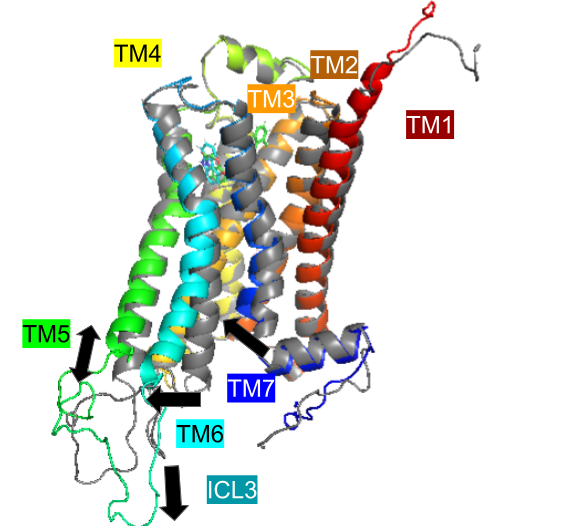
\includegraphics[width=\textwidth]{system-all-with-label.png}
    \caption{$\beta_2$ARのTM5,TM6,TM7の変化。}
    \label{fig:fitting_TM}
  \end{subfigure}
  \hspace{0.02\textwidth} % 図の間のスペース
  \begin{subfigure}{0.88\textwidth}
    \centering
    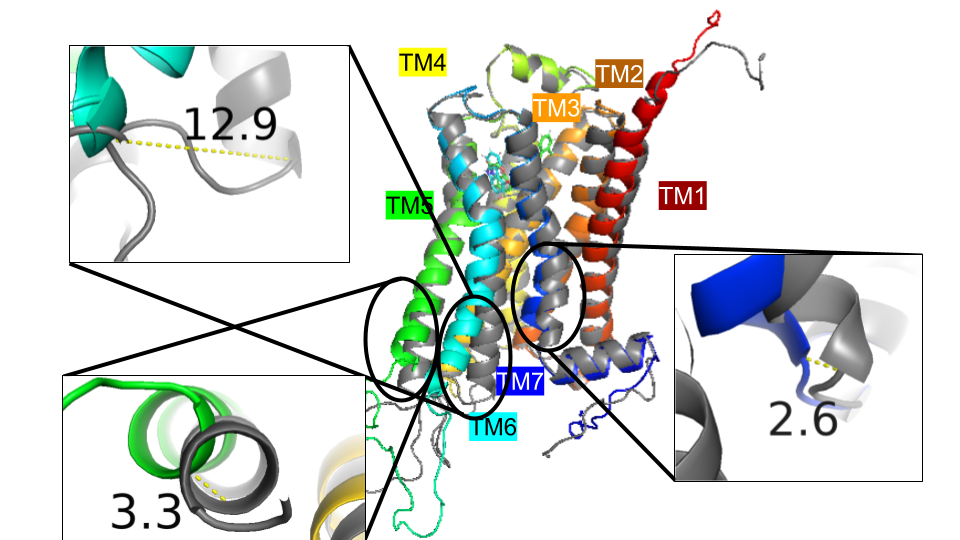
\includegraphics[width=\textwidth]{system-all-with-label-detail.png}
    \caption{$\beta_2$ARのTM5,TM6,TM7の変化の詳細。}
    \label{fig:fitting_TM_detail}
  \end{subfigure}
  \caption{$\beta_2$ARのinactive構造(灰色)とactive構造(色付き)の重ね合わせ。}
  \label{fig:fitting-all}
\end{figure}

\newpage

TM6の細胞質側末端にある残基の$\mathrm{C}_\alpha$原子が、TM7から離れる方向に12.9Å移動する様子が観察された。
TM5の細胞質側末端部分は末端の$\mathrm{C}_\alpha$原子がTM3から離れる方向に3.3Å移動する様子が観察された。
TM7の細胞質側末端にある残基の$\mathrm{C}_\alpha$原子が、タンパク質の内側に近づく方向に2.6Å移動する様子が観察された。
TM5とTM6を結ぶ細胞内ループ3(ICL3)においても、Gタンパク質結合部位を開くように特定の方向に並んでいるような様子が観察された。


\subsubsection{$\beta_2$ARの保存された結晶水}
DOWSERによって検出された、エネルギー的に安定な水分子は、inactive状態で14869個、active状態で18876個同定された。
そのうち、シミュレーション中で保存されている結晶水はinactive状態で7個、active状態で6個同定された。

\begin{figure}[htbp]
    \centering
    \begin{subfigure}{0.48\textwidth} % 各図の幅を調整
      \centering
      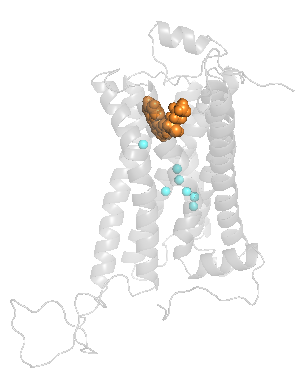
\includegraphics[width=\textwidth]{inactive_saved_water.png}
      \caption{$\beta_2$ARのinactive状態における保存された結晶水。}
      \label{fig:inactive_water}
    \end{subfigure}
    \hspace{0.02\textwidth} % 図の間のスペース
    \begin{subfigure}{0.48\textwidth}
      \centering
      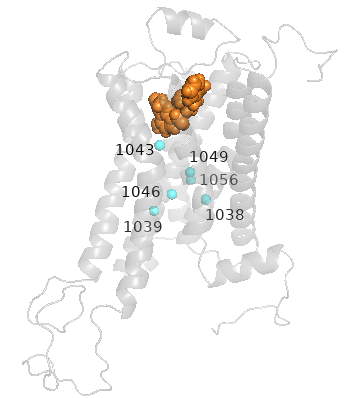
\includegraphics[width=\textwidth]{active_saved_water.png}
      \caption{$\beta_2$ARのactive状態における保存された結晶水。}
      \label{fig:active_water}
    \end{subfigure}
    \caption{保存された結晶水}
    \label{fig:water-all}
  \end{figure}

\newpage

%inactiveとactiveで保存されている結晶水
シミュレーション中で保存されているinactive状態の7個の結晶水、active状態の6個の結晶水のうち、
双方で共通の位置に存在していた結晶水は4つあったため、残基番号をそれぞれ(344,346,347,348)と定めた。
それ以外の結晶水は、(355,356,357,358,359)の残基番号を振り分けた。

\begin{figure}[htbp]
  \centering
  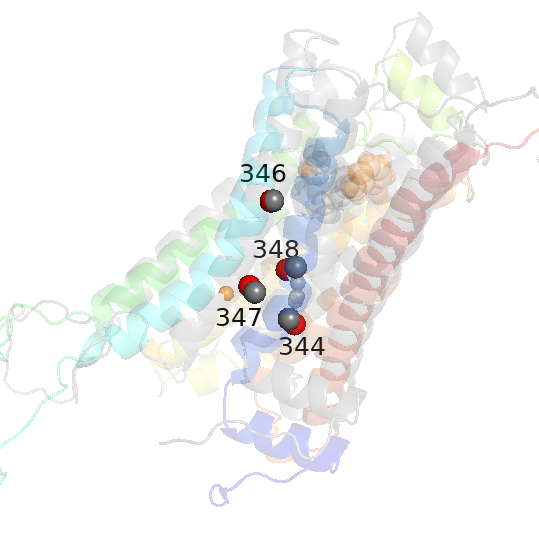
\includegraphics[width=0.8\textwidth]{xwater_fitting.png}
  \caption{保存された結晶水のうち、$\beta_2$ARのinactive状態とactive状態の双方で共通の位置に存在する水分子。}
  \label{fig:xwater_fitting}
\end{figure}

\newpage

%水分子、先行研究との比較

\section{$\beta_2$ARのinactiveおよびactive状態のコミュニティ検出}

得られた座標データを基に、ネットワークのエッジの重みとして用いる残基間最短距離の2乗逆数の平均$\langle \frac{1}{d^2} \rangle$ を計算した。

エッジを以下の条件で形成させた後、エッジの重みを加え、inactive状態active状態双方のネットワークを構築した。
1. 残基ペア間の最短距離が3\,\text{\AA}未満である場合、エッジを形成する。
2. アミノ酸配列上で隣接する残基感のエッジは削除する。

以下が構築されたネットワークの詳細である。
\begin{table}[!ht]
    \centering
    \caption{ネットワーク上のノード数と、残基ペア間の最短距離が3\,\text{\AA}未満のエッジ数}
    \begin{tabular}{lll}
      \hline
      モデル名          & ノード数  & エッジ数 \\
      \hline 
      inactive(2RH1)  &  351 &  16332 \\ 
      active(3P0G)    &  349 &  15433 \\ 
    \end{tabular}
    \label{tab:network_size}
  \end{table}

構築されたネットワークを基に、コミュニティ検出を行った。
\subsubsection{Louvain法の信頼性}

ネットワークにおけるコミュニティ構造を検出するために用いたLouvain法の結果の信頼性は、モジュラリティ$Q$の値を用いて評価される。
モジュラリティ$Q$の値は通常-1から1の範囲を取り、以下のように解釈される:

\begin{itemize}
    \item \( Q \) が負:分割がネットワーク構造と一致しておらず、不適切な分割である。
    \item \( Q \) が 0 に近い:ネットワークがランダム構造に近い。
    \item \( Q \) が正:ネットワーク内にコミュニティ構造が存在する。
\end{itemize}

本研究の解析対象である$\beta_2$ARのinactiveおよびactive状態のコミュニティ検出におけるモジュラリティ$Q$の最良値および標準偏差を計算した。

\paragraph{試行回数100回におけるモジュラリティ値の平均および標準偏差}
\begin{itemize}
    \item inactive状態: \( Q = 0.5163 \pm 0.0054 \)
    \item active状態: \( Q = 0.5239 \pm 0.0044 \)
\end{itemize}
さらに、モジュラリティ値の標準誤差は以下の通りです:
\begin{itemize}
    \item inactive状態: \( \pm 0.0005 \)
    \item active状態: \( \pm 0.0004 \)
\end{itemize}

inactive状態とactive状態のモジュラリティ値はどちらも正の値を示しており、ネットワーク内に明確に分割されたコミュニティ構造があることを示唆している。

\subsection{Louvain法で検出されたコミュニティ}

以下に$\beta_2$ARのinactive構造とactive構造で検出されたコミュニティを示す。

\begin{figure}[htbp]
    \centering
    \begin{subfigure}{0.60\textwidth} % 各図の幅を調整
      \centering
      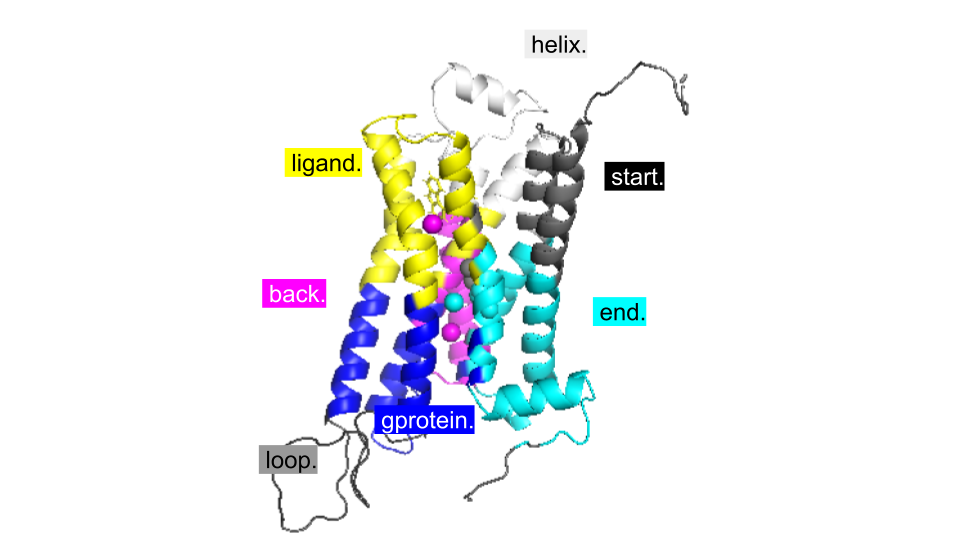
\includegraphics[width=\textwidth]{inactive_with_label.png}
      \caption{inactive状態において検出されたコミュニティ構造を色分けして示した図。各色と名付けたコミュニティは以下に表す:黒(start)、シアン(end)、白(helix)、ピンク(back)、グレー(loop)、黄色(ligand)、青(gprotein)。}
      \label{fig:inactive_community}
    \end{subfigure}
    \hspace{0.02\textwidth} % 図の間のスペース
    \begin{subfigure}{0.60\textwidth}
      \centering
      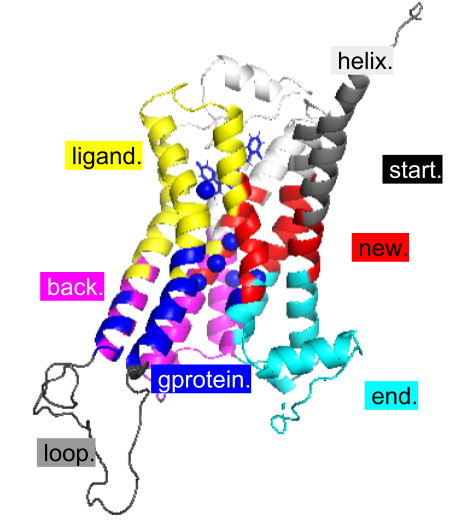
\includegraphics[width=\textwidth]{active_with_label.png}
      \caption{active状態において検出されたコミュニティ構造を色分けして示した図。各色と名付けたコミュニティは以下に表す:黒(start)、シアン(end)、白(helix)、ピンク(back)、グレー(loop)、黄色(ligand)、青(gprotein)、赤(new)。}
      \label{fig:active_community}
    \end{subfigure}
    \caption{$\beta_2$ARのLouvain法で検出されたコミュニティ構造}
    \label{fig:community-all}
  \end{figure}

\newpage

まず双方のコミュニティに共通することとして、リガンド結合部位と活性部位であるGタンパク質結合部位に対応する独立したコミュニティが、黄色(ligand)、青(gprotein)として検出された。
またinactive状態からactive状態への変化として、青(gprotein)コミュニティの再編成が起きていることと、赤(new)コミュニティが新規に形成されたことが挙げられる。

\begin{table}[!ht]
  \centering
  \caption{活性化に伴うコミュニティの再編成と、コミュニティを構成している残基群の比較}
  \resizebox{\textwidth}{!}{
    \begin{tabular}{lll}
      \hline
      活性化に伴うコミュニティの再編成  & inactiveでの構成要素  & activeでの構成要素 \\
      \hline 
      青(gprotein)コミュニティの再編成  &  TM3,TM5,TM6の細胞質側残基  &  TM6の細胞質側残基、リガンド、6つの保存された結晶水 \\
      赤(new)コミュニティの新規形成  &  なし  & TM7,TM1,TM2の中間付近に位置する残基 \\ 
    \end{tabular}
  }
  \label{tab:community_change}
\end{table}

青(gprotein)コミュニティの再編成が起きたのは、
TM5,TM6の細胞質側がタンパク質の中心から離れるように外側に動いたことで、
もともと同じ青(gprotein)コミュニティに所属していたTM3と別のコミュニティに分かれたためだと考えられる。
実際にTM6の顕著な動きにより、TM5とTM6が協調して動くことが確認されている。
%https://pubs.acs.org/doi/full/10.1021/jp506579a
しかしその独立したTM6の青(gprotein)コミュニティに、active状態に存在している保存された結晶水6つ全てとリガンドが含まれたことは興味深い結果であり、
これと、赤(new)コミュニティの新規形成が、シグナル伝達経路にどう影響を与えるかは以後の分析で考察していくこととする。
%コミュニティが1つ増えることに言及はしているが、コミュニティの解析はしていない
%https://pubs.acs.org/doi/full/10.1021/jp506579a

ここで、inactive状態とactive状態で示されているネットワークの全体密度を計算する。
全体エッジ密度$D_{\text{global}}$の計算式は以下のように表される。

\begin{equation}
W_{\text{actual}} = \sum_{(u, v) \in E} w(u, v)
\end{equation}

$W_{\text{actual}}$は実際のエッジ重みの合計である。
$E$は、グラフ内のエッジ集合を示す。
$w(u, v)$は、エッジ$(u, v)$の重みを示す。

\begin{equation}
W_{\text{max}} = \sum_{i=1}^{N} \sum_{j=i+1}^{N} w(i, j)
\end{equation}

$W_{\text{max}}$は理論上可能な最大エッジ重みの合計である。
$N$は、グラフ内のノード数を示す。
$w(i, j)$は、ノード$i$と$j$の間のエッジ重みを示す。

\begin{equation}
D_{\text{global}} = \frac{W_{\text{actual}}}{W_{\text{max}}}
\label{eq:global_density}
\end{equation}

最終的に、ネットワークの全体エッジ密度$D_{\text{global}}$は以上のように示される。

この式に基づいて、inactive構造とactive構造のネットワークの全体エッジ密度を計算すると、それぞれ以下のようになる。
\begin{itemize}
    \item inactive状態:\( D = 0.3086 \)
    \item active状態:\( D = :0.8579 \)
\end{itemize}

inactive状態の方がエッジ数、つまり最短距離が3\,\text{\AA}未満の残基ペアが多いにも関わらず、存在するエッジの重みの合計が小さかった。
それに対しactive状態は、inactive状態に比べてエッジ数、つまり最短距離が3\,\text{\AA}未満の残基ペアが少ないにも関わらず、存在するエッジの重みの合計が大きく、高い全体エッジ密度となった。
この結果は、active状態になると近接した残基ペアが増加し、タンパク質の構造がより密接にパッキングされることを示唆している。

\subsection{コミュニティ内およびコミュニティ間のエッジ密度}
active状態で再編成されたコミュニティや新しく検出されたコミュニティの役割を定量的に分析するために、ネットワークの全体密度$D_{\text{global}}$の計算で用いた密度の概念を用いたさらなる計算を行った。
続いて、inactive状態とactive状態双方においてそれぞれコミュニティ内のエッジ密度、コミュニティ間のエッジ密度を計算した。

\subsubsection{コミュニティ内エッジ密度}
コミュニティ内エッジ密度$D_{\text{internal}}$の計算式は以下のように表される。

まずコミュニティごとにサブグラフを作成する。
ただしコミュニティ間のエッジは削除し、独立したコミュニティを表現している。
続いてコミュニティ内エッジ密度を計算する。

\begin{equation}
D_{\text{internal}} = \frac{\sum_{(u,v) \in E_C} w_{uv}}{\sum_{(u,v) \in E_C} w_{uv}^{\text{max}}}
\label{eq:internal_density}
\end{equation}

ここで$E_C$はコミュニティ$C$内の全エッジの集合、$w_{uv}$はノード$u$とノード$v$の間の実際のエッジ重み、$w_{uv}^{\text{max}}$はノード$u$とノード$v$の間のエッジの最大可能重みである。

分子の$\sum_{(u,v) \in E_C} w_{uv}$はコミュニティに属するノード間に存在する実際のエッジの重みの合計を示している。
分母の$\sum_{(u,v) \in E_C} w_{uv}^{\text{max}}$は、
そのコミュニティ内の全てのノードが完全に接続している場合のエッジの最大可能重みの合計を示している。

ただし、自己ループは除く。


コミュニティ内エッジ密度$D_{\text{internal}}$は、ネットワーク全体のエッジ密度を基準としてコミュニティ内のエッジ密度がネットワーク全体と比べて相対的にどれだけ高い(または低い)かを示し、コミュニティ内部でどれだけ密接に関連しているかを測定することを目的としている。
上記の式に基づいて、inactive構造とactive構造のコミュニティ内エッジ密度を計算すると、それぞれ以下のようになる。

\begin{figure}[htbp]
    \centering
    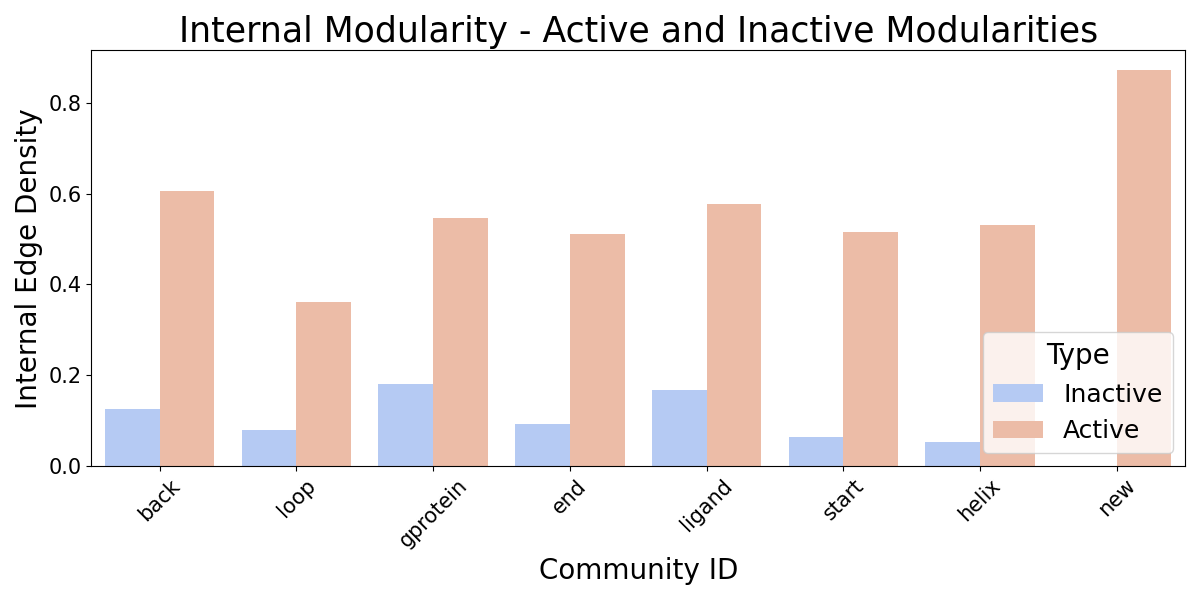
\includegraphics[width=1.0\textwidth]{internal_modularities.png}
    \caption{$\beta_2$ARのinactive状態とactive状態において検出されたコミュニティのコミュニティ内エッジ密度を示した図。コミュニティの名称は、コミュニティ構造で名付けたものである。}
    \label{fig:internal}
\end{figure}

\newpage

コミュニティ内エッジ密度$D_{\text{internal}}$の値は以下のように解釈される:
\begin{itemize}
    \item \( D_{\text{internal}} \) が 0 に近い:コミュニティ内のノード間の相互作用は希薄であり、結びつきが弱い。
    \item \( D_{\text{internal}} \) が 1 に近い:コミュニティ内のノード間には強い結びつきがあり、密に相互作用している。
\end{itemize}

inactive構造では、end, ligand, startコミュニティのコミュニティ内エッジ密度が、相対的に低い値を示した。
しかしactive構造で新たに出現したnewコミュニティと共に、全てのコミュニティのコミュニティ内エッジ密度が1.0付近という値を示した。
活性化に伴って、すべてのコミュニティの内部が強い結びつきを形成している構造に変化したことがわかる。

\subsubsection{コミュニティ間エッジ密度}
コミュニティ間エッジ密度$D_{\text{inter}}$の計算式は以下のように表される。

\begin{equation}
D_{\text{inter}} = \frac{\sum_{\substack{u \in C_i \\ v \in C_j}} w_{uv}}{\sum_{\substack{u \in C_i \\ v \in C_j}} w_{uv}^{max}}
\label{eq:inter_density}
\end{equation}

ここで $C_i$ と $C_j$ はそれぞれ異なるコミュニティ $i$ と $j$、$w_{uv}$ はノード $u$ とノード $v$ の間の実際のエッジ重み、$w_{uv}^{\text{max}}$ はノード $u$ とノード $v$ の間のエッジの最大可能重みである。
分子の $\sum\limits_{\substack{u \in C_i \\ v \in C_j}} w_{uv}$ は異なるコミュニティに属するノード間の実際のエッジの重みの合計を示している。
分母の $\sum\limits_{\substack{u \in C_i \\ v \in C_j}} w_{uv}^{\text{max}}$ は、そのコミュニティ間の全てのノードが完全に接続している場合のエッジの最大可能重みの合計を示している。
ただし、自己ループは除く。

コミュニティ間エッジ密度は、異なるコミュニティ間のエッジの結びつきの強さを示しており、お互いにどれだけ相互作用が強いかを測定することを目的としている。
上記の式に基づいて、inactive構造とactive構造のコミュニティ間エッジ密度を計算すると、それぞれ以下のようになる。

\begin{figure}[htbp]
    \centering
    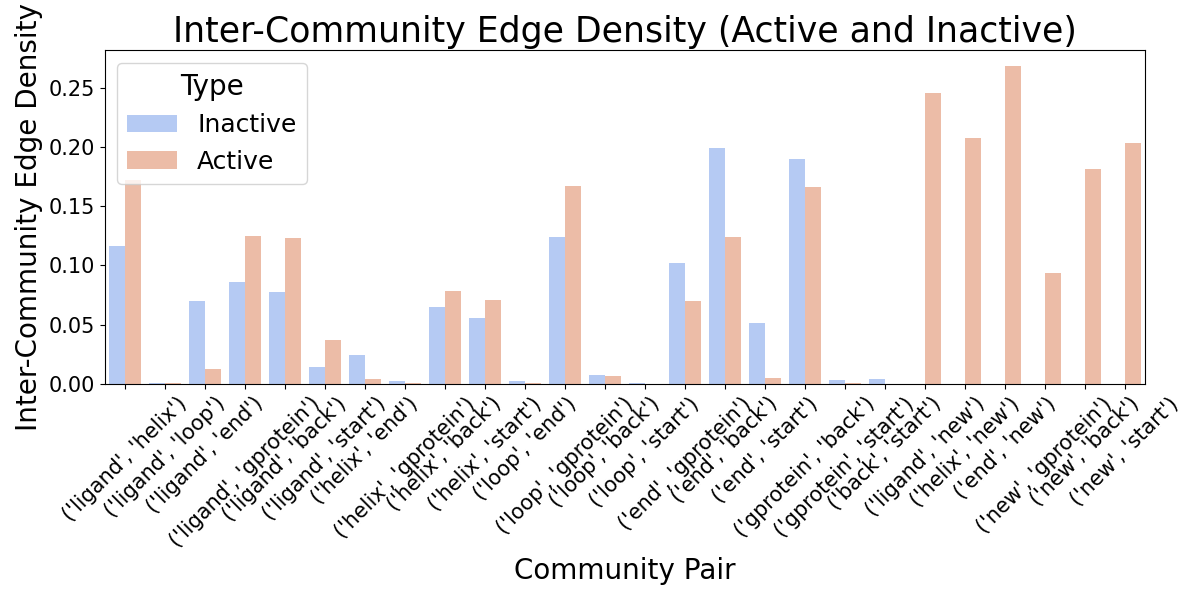
\includegraphics[width=1.0\textwidth]{interedge_modularities.png}
    \caption{$\beta_2$ARのinactive状態とactive状態において検出されたコミュニティのコミュニティ間エッジ密度を示した図。コミュニティの名称は、コミュニティ構造で名付けたものである。}
    \label{fig:inter}
\end{figure}

\newpage

ただし、inactive状態とactive状態の双方でコミュニティ間エッジ密度が0だったコミュニティペアは、図から除外している。
該当するコミュニティペアはstart-loop、helix-loop、new-loopである。

コミュニティ間エッジ密度$Q$の値は以下のように解釈される:
\begin{itemize}
    \item \( Q \) が 0 に近い:コミュニティ間でエッジが少なく、各コミュニティがほぼ独立している。
    \item \( Q \) が 1 に近い:コミュニティ間で多数のエッジが存在し、コミュニティ間の結びつきが強い。
\end{itemize}

inactive状態では最も高い値で0.52であったのが、
active状態になると15ものコミュニティペアが、0.5以上の値をとった。
そのうちnewに関わるコミュニティペアは6つ、gproteinは5つ、backとligandはそれぞれ4つ含まれていた。

inactive構造からactive構造へのコミュニティ間エッジ密度の変化を以下に示した。

\begin{figure}[htbp]
  \centering
  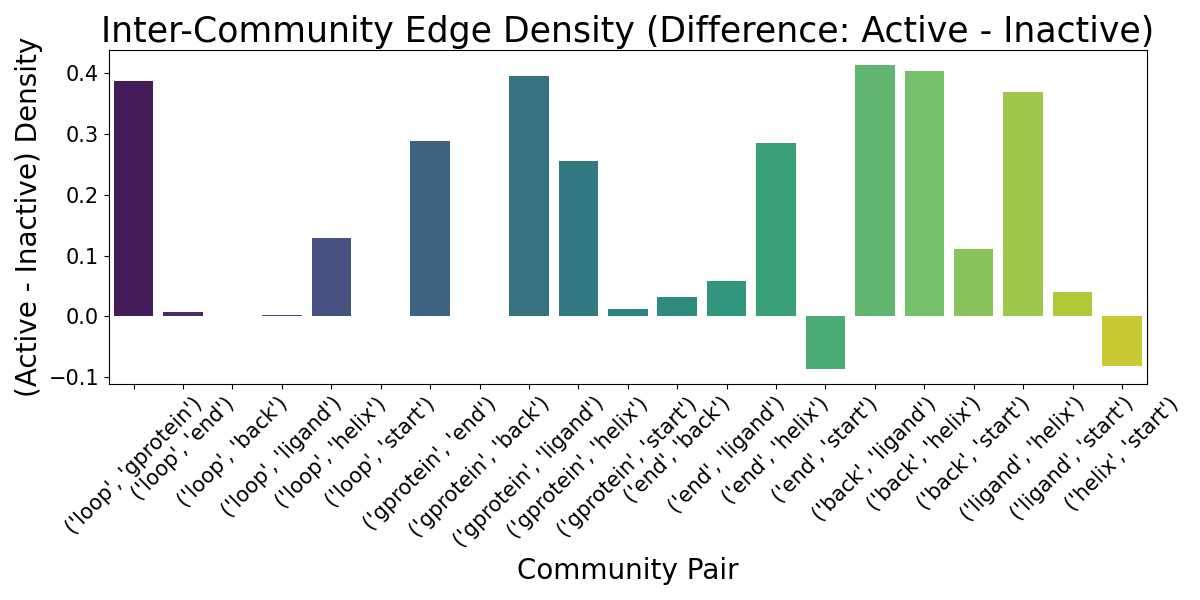
\includegraphics[width=1.0\textwidth]{interedge_modularities_diff.png}
  \caption{$\beta_2$ARの各コミュニティのコミュニティ間エッジ密度の変化を示した図。コミュニティの名称は、コミュニティ構造で名付けたものである。}
  \label{fig:inter_diff}
\end{figure}

\newpage

リガンド結合部位と活性部位を結ぶ経路上のコミュニティペア(loop-gprotein,gprotein-ligand,back-ligand,back-helix,ligand-helix)のコミュニティ間エッジ密度が0.35以上変化したことがわかる。

\subsubsection{inactive状態とactive状態の全体密度、コミュニティ密度の考察}


\paragraph{密度に関わる3つの変数における、inactive状態からactive状態への変化}

ここまでinactive状態とactive状態のコミュニティ内エッジ密度、コミュニティ間エッジ密度、全体エッジ密度の変化を通じて、コミュニティ内およびコミュニティ間の相互作用を定量的に評価してきた。
それぞれ、以下のことが示唆される。
\begin{enumerate}
  \item \textbf{全体エッジ密度の増加}: active状態への遷移に伴い、ネットワーク全体のエッジ密度が増加した。これにより、分子全体の協調的な相互作用が強化され、アロステリック遷移の効率が向上したと考えられる。
  \item \textbf{コミュニティ内エッジ密度の増加}: active状態では、すべてのコミュニティ内エッジ密度が1.0付近という高い値を示した。これは、活性化に伴い、各コミュニティ内部で強固な相互作用が形成され、分子内の情報伝達の効率が向上したことを示している。
  \item \textbf{コミュニティ間エッジ密度の増加}: active状態において、コミュニティ間エッジ密度が大幅に増加し、特に新しく生成されたnewコミュニティに関連するコミュニティペアは高い値を示した。これにより、異なるコミュニティ間の協調的な情報伝達が強化され、分子全体の相互作用ネットワークが再編成されたことが示唆される。
\end{enumerate}

これらの結果は、active状態への遷移に伴う分子全体のネットワーク再編成が、分子内情報伝達の効率化を支える重要なメカニズムであることを示している。
特に、newコミュニティが形成されたことで、リガンド結合部位と活性部位間の情報伝達が促進されている点を考慮すると、
リガンド結合部位や活性部位であるGタンパク質結合部位間の情報伝達を促進する導管として働いている可能性があることが示唆された。
このことは、アロステリック遷移における協調的な相互作用の重要性を示唆しており、分子内情報伝達の動的メカニズム解明に貢献するものと考えられる。

(密度変化やnewコミュニティの重要性や生理的・機能的意義を、先行研究と交えて)
%先行研究

ここまで、コミュニティ内外のエッジ密度の変化に基づき、active状態への遷移に伴う分子全体のネットワーク再編成について議論してきた。
しかし、コミュニティ単位の相互作用だけでは、各ノードが分子全体の接続性や情報伝達にどのように寄与しているのかを十分に把握することはできない。
そこで、次にノード単位でのコミュニティに与える影響を詳細に分析し、分子内のネットワークの構造や情報伝達効率への貢献度を評価する。


\section{ノード削除によるactiveネットワーク接続性への影響}

あるノードがactiveネットワーク全体または所属するコミュニティの接続性に与える影響を定量化に評価するために、impact scoreという変数を導入した。
これは、特定のノードをactiveネットワークから削除した際に生じる全体エッジ密度とコミュニティ内エッジ密度の変化量を基に計算した。
全体エッジ密度とコミュニティ内エッジ密度はそれぞれ前述の式に従っている。
以降、全体エッジ密度の変化量をglobal impact score、コミュニティ内エッジ密度の変化量をcommunity impact scoreと表現する。

また、global impact scoreとcommunity impact scoreについて、Zスコアを算出することで影響の大小を統計的に評価する。
Zスコアは、あるデータ点で平均からどれだけ標準偏差の単位で離れているかを示す指標である。Zスコアの計算式は以下のとおりである。

\begin{equation}
z = \frac{x - \mu}{\sigma}
\end{equation}

ここで$x$はデータ点の値、$\mu$はデータセットの平均、$\sigma$はデータセットの標準偏差を示している。
Zスコアの解釈は以下のとおりである。
\begin{itemize}
    \item \( z < 0 \):データ点は平均よりも小さい値である。
    \item \( z = 0 \):データ点は平均と一致している。
    \item \( z > 0 \):データ点は平均よりも大きい値である。
    \item \( z > 2 \):データ点は平均から2標準偏差以上離れており、全体の約2.5\%にあたるくらい高い値である。
\end{itemize}

\subsubsection{global impact score}
global impact scoreの変化量が大きかったノードのうち、Zスコアが2以上であったノードを昇順に並び替えたのが以下の表である。
\begin{table}[ht]
    \centering
    \begin{tabular}{|l|r|c|r|}
    \hline
    \textbf{Node} & \textbf{Global Impact Score} & \textbf{Community} & \textbf{Node type}\\
    \hline
    303 & 0.000776 & new & Ligand-Site \\
    62 & 0.000774 & new & Other \\
    66 & 0.000767 & new & Motif \\
    273 & 0.000754 & ligand & Motif \\
    111 & 0.000748 & new & Other \\
    96 & 0.000741 & helix & Ligand-Site \\
    69 & 0.000740 & new & Motif \\
    107 & 0.000724 & new & Motif \\
    104 & 0.000684 & new & Ligand-Site \\
    108 & 0.000678 & ligand & Other \\
    58 & 0.000670 & back & Other \\
    100 & 0.000648 & new & Ligand-Site \\
    347 & 0.000641 & gprotein & X-Water \\
    105 & 0.000640 & helix & Ligand-Site \\
    110 & 0.000636 & back & Other \\
    339 & 0.000635 & end & Other \\
    114 & 0.000627 & back & Other \\
    186 & 0.000623 & helix & Ligand-Site \\
    \hline
    \end{tabular}
    \caption{Top 18 Nodes by Impact Score}
\end{table}

\newpage

ここでCommunityの名称は、コミュニティ構造で名付けたものである。
%Node typeの説明

上位10このうち7このノードがnewコミュニティに属しており、active構造で検出された新しいコミュニティがタンパク質全体に重要な役割を果たしていることが示唆された。
また、ligand,newコミュニティに属しているモチーフに関連するノードも上位10このうち4こ存在しており、これらの領域が全体のネットワーク密度に強い影響を与えていることが示唆される。
%リガンド結合が受容体の活性化に伴う全体的な構造変化を引き起こすという既存の知見
%https://www.cosmobio.co.jp/aaas_signal/archive/ra-20200204-2.asp?utm_source=chatgpt.com

\subsubsection{community impact score}
community impact scoreが大きかったノードのうち、Zスコアが2以上であったノードを昇順に並び替えたのが以下の表である。
\begin{table}[ht]
    \centering
    \begin{tabular}{|l|r|c|r|}
    \hline
    \textbf{Node} & \textbf{Community Impact Score} & \textbf{Community} & \textbf{Node type}\\
    \hline
    347 & 0.002869 & gprotein & X-Water \\
    346 & 0.002752 & gprotein & X-Water \\
    348 & 0.002677 & gprotein & X-Water \\
    356 & 0.002664 & gprotein & X-Water \\
    343 & 0.002604 & gprotein & Ligand \\
    241 & 0.002372 & loop & Other \\
    258 & 0.002274 & gprotein & Gprotein-Site \\
    1 & 0.002248 & start & Other \\
    355 & 0.002233 & gprotein & X-Water \\
    259 & 0.002149 & gprotein & Other \\
    231 & 0.002121 & loop & Other \\
    243 & 0.002047 & loop & Other \\
    236 & 0.001998 & loop & Other \\
    17 & 0.001990 & start & Other \\
    242 & 0.001974 & loop & Other\\
    239 & 0.001962 & loop & Other \\
    2 & 0.001876 & start & Other \\
    255 & 0.001870 & gprotein & Motif \\
    222 & 0.001826 &  loop & Other \\
    261 & 0.001806 & gprotein & Gprotein-Site \\
    260 & 0.001784 & gprotein & Other \\
    339 & 0.001767 & end & Other \\
    217 & 0.001761 & loop & Gprotein-Site \\
    \hline
    \end{tabular}
    \caption{Top 23 Nodes by Impact Score}
\end{table}
  
\newpage

23このうち18このノードがgprotein,loopコミュニティに属しており、活性化による構造変化が見られたTM5,TM6,TM7の細胞質側領域とICL3がここに含まれていることから、
gprotein,loopコミュニティに属する残基がコミュニティ内の重要な結束性に寄与している可能性があることが示唆された。
また、保存された結晶水が上位10このうち5つを占めており、保存された結晶水がGタンパク質結合領域内で強い影響力を持つことを示している。
%Gタンパク質の活性化には、受容体の特定の構造変化が必要であり、これらの局所的な相互作用がそのプロセスを制御している可能性
%https://seikagaku.jbsoc.or.jp/10.14952/SEIKAGAKU.2022.940916/data/index.html?utm_source=chatgpt.com
%選択的活性化
%https://www.cosmobio.co.jp/aaas_signal/archive/ra-20200204-2.asp?utm_source=chatgpt.com


\subsubsection{global impact score、community impact scoreの考察}

global impact scoreが目立った残基は、ネットワーク全体の構造を保つ役割を果たしていると推測される。
つまり、global impact scoreが高かったnewコミュニティに属する残基やモチーフは、ネットワーク全体の「骨格」としてリガンド結合によるネットワーク全体の再編成を保っており、アロステリックな影響を広げる重要な起点となっていることが示唆される。
一方でcommunity impact scoreが目立った残基は、局所的なコミュニティ構造を保つ役割を果たしていると推測される。
つまり、gprotein,loopコミュニティに属する残基や、保存された結晶水は局所的な「足場」を提供し、Gタンパク質の結合やシグナル伝達の効率化を高めていることが示唆される。



%\section{シグナル伝達機構の考察}
%(以下は、完全に仮説なので、この仮説を裏付ける先行研究が発見されなければ、削除)

%ここまでinactive状態とactive状態におけるコミュニティ内密度とコミュニティ間密度、active状態のネットワークにおけるノードがactiveネットワーク全体または所属するコミュニティの接続性に与える影響について解析をしてきた。
%これらの解析結果を踏まえると、以下のような段階的なシグナル伝達機構が考えられる。

%まずリガンドがリガンド結合部位に結合すると、まず結合近傍の局所的なコミュニティ再編成が起きる。
%この再編成はリガンドが高いcommunity impact scoreを示したことに反映されている
%続いて再編成されたリガンド結合部位が、局所的な変化を他のコミュニティへと伝播させることで、ネットワーク全体の構造変化が促進される。
%この過程は、ligandコミュニティと他のコミュニティにおけるコミュニティ間密度が大幅に増加したことや、リガンド結合部位が高いglobal impact scoreを示したことに反映されている。
%最後に、再編成されたネットワーク全体がgタンパク質結合部位や保存された結晶水などの局所的な結束性によって安定化され、シグナル伝達が効率的に進む。
%この過程は、gproteinコミュニティのコミュニティ内密度が大幅に増加したことや、gproteinコミュニティに含まれる保存された結晶水が高いcommunity impact scoreを示したことに反映されている。